\documentclass[11pt,a4paper]{article}

% ------------------------------------------------------------------
% Packages
% ------------------------------------------------------------------
\usepackage{amsmath, amssymb}
\usepackage{graphicx}
\usepackage{booktabs}
\usepackage{siunitx}        % better tables
\usepackage{hyperref}
\usepackage{authblk}        % author + affiliation
\usepackage[margin=2.5cm]{geometry}

% ------------------------------------------------------------------
% Metadata
% ------------------------------------------------------------------
\title{Aerial--Image Cactus Identification with a Compact Convolutional Neural Network}

\author[1]{Juan~David~Zapata~Cruz}
\author[2]{Krisostomus~Nova~Rahmanto}
\author[3]{Kristian~H{\aa}land}
\affil[1]{Department of Computer Science, University A}
\affil[2]{School of Electrical Engineering, University B}
\affil[3]{Institute of Environmental Modelling, University C}

\date{May 2025}

% ------------------------------------------------------------------
\begin{document}
\maketitle

% ------------------------------------------------------------------
\begin{abstract}
Accurate detection of \textit{Cereus} cacti in ultra--low--resolution aerial imagery supports desert ecosystem monitoring and invasive--species management, yet the task is challenging owing to severe class imbalance and limited spatial detail.  
We propose a deliberately lightweight convolutional neural network (CNN) tailored to \SI{32 x 32}{\pixel} RGB photographs supplied by the \emph{Aerial Cactus Identification Challenge}.  
Trained with targeted data augmentation and modest regularisation, the model attains \textbf{99.1\,\% overall accuracy, an F\textsubscript{1}--score of 0.98, and an AUC--ROC of 0.98} on a withheld test set, while requiring only $1.7\times 10^{5}$ trainable parameters.  
The results demonstrate that a carefully‐designed, low‐latency architecture suffices for near‐perfect binary classification in this domain and serves as a practical baseline for large‐scale UAV deployments.
\end{abstract}

% ------------------------------------------------------------------
\section{Introduction}\label{sec:intro}

Unmanned–aerial–vehicle (UAV) missions now acquire thousands of images per sortie, enabling near–real‐time surveillance of fragile desert habitats.  
Manual annotation is both time–consuming and error‐prone, motivating automatic detectors that can flag cactus presence with minimal human oversight.  
Although deep CNNs dominate modern image recognition, most architectures exceed \num{10}~million parameters and target megapixel imagery.  
This study shows that such complexity is unnecessary for the constrained scenario of \SI{32 x 32}{\pixel} aerial tiles.

We cast cactus identification as a binary classification problem
%
\[
f : \mathbb{R}^{32\times 32 \times 3} \longrightarrow \{0,1\}, 
\qquad 
y = 1 \iff \text{cactus present}.
\]
%
Our contributions are three‐fold:
\begin{enumerate}
  \item A compact CNN architecture specifically adapted to extremely low resolution;
  \item A training pipeline that mitigates class imbalance without explicit re‐weighting; and
  \item An empirical evaluation showing a favourable performance–efficiency trade‐off.
\end{enumerate}

% ------------------------------------------------------------------
\section{Dataset and Pre‐processing}\label{sec:data}

The public dataset comprises \num{17\,500} JPEG images of dimension \SI{32 x 32 x 3}{\pixel}, of which roughly \SI{75}{\percent} contain at least one cactus.  
We adopt a stratified split of \SI{60}{\percent} training, \SI{20}{\percent} validation, and \SI{20}{\percent} testing to preserve the prior class distribution.

\paragraph{Normalisation.}
Pixel intensities are rescaled linearly to $[0,1]$.

\paragraph{Data augmentation.}
At training time, each mini‐batch is perturbed by random horizontal and vertical flips, rotations up to $\pm20^{\circ}$, and width/height shifts or zooms of at most \SI{10}{\percent}.  
These transforms enlarge the effective data manifold six‐fold and combat over‐fitting without altering semantic content.

% ------------------------------------------------------------------
\section{Methodology}\label{sec:method}

\subsection{Network Architecture}

Figure~\ref{fig:architecture} illustrates the eight‐layer CNN used in this work:

\begin{center}
\begin{tabular}{ll}
\toprule
\textbf{Layer} & \textbf{Specification} \\
\midrule
Input          & \SI{32 x 32 x 3}{\pixel} \\[2pt]
Conv2D         & $32$ filters, $3\times3$, ReLU \\ 
MaxPooling     & $2\times2$ \\[2pt]
Conv2D         & $64$ filters, $3\times3$, ReLU \\ 
MaxPooling     & $2\times2$ \\[2pt]
Flatten        & --- \\
Dense          & $64$ units, ReLU \\
Dropout        & $p=0.3$ \\
Dense (output) & $1$ unit, sigmoid \\
\bottomrule
\end{tabular}
\end{center}

The model contains $1.7 \times 10^{5}$ parameters, balancing representation power and inference speed.

\subsection{Training Protocol}

\begin{itemize}
  \item \textbf{Loss / optimiser}  Binary cross‐entropy minimised with Adam ($\mathrm{lr}=10^{-3}$).
  \item \textbf{Batch size}  $64$.
  \item \textbf{Epochs}  $15$ epochs with early stopping (patience $=3$).
  \item \textbf{Learning–rate schedule}  \texttt{ReduceLROnPlateau} halves the learning rate when validation loss stalls.
\end{itemize}

Dropout in the penultimate layer provides the sole explicit regulariser; batch normalisation was empirically unnecessary.

% ------------------------------------------------------------------
\section{Experimental Results}\label{sec:results}

\subsection{Learning Dynamics}

Validation accuracy converges to \SI{98}{\percent} within ten epochs, and the final training–validation gap remains below one percentage point (Figure~\ref{fig:learning}), indicating limited over‐fitting.

\subsection{Quantitative Evaluation}

\begin{table}[h]
  \centering
  \caption{Test–set performance metrics.}
  \label{tab:metrics}
  \begin{tabular}{lc}
    \toprule
    \textbf{Metric} & \textbf{Value} \\
    \midrule
    Accuracy  & 0.991 \\
    Precision & 0.980 \\
    Recall    & 0.999 \\
    F\textsubscript{1}–score & 0.988 \\
    AUC–ROC   & 0.977 \\
    \bottomrule
  \end{tabular}
\end{table}

\begin{table}[h]
  \centering
  \caption{Confusion matrix on the held‐out test set.}
  \label{tab:confusion}
  \begin{tabular}{lcc}
    \toprule
               & \multicolumn{2}{c}{\textbf{Predicted}}\\
    \cmidrule{2-3}
    \textbf{True}   & No cactus & Cactus \\
    \midrule
    No cactus & 843 & 30  \\
    Cactus    & 3   & 2\,595 \\
    \bottomrule
  \end{tabular}
\end{table}

Only three cacti are missed, while thirty non‐cactus tiles are incorrectly flagged, yielding a recall suitable for ecological applications where false negatives are costly.

% ------------------------------------------------------------------
\section{Discussion}\label{sec:discussion}

The study underlines three key insights:

\begin{enumerate}
  \item \textbf{Sufficiency of light architectures} -- For \SI{32}{\pixel} inputs, deeper backbones provide diminishing returns versus their computational cost.  
  \item \textbf{Implicit imbalance handling} -- Simple augmentation and dropout restore balanced performance without class weighting or focal loss.  
  \item \textbf{Deployability} -- The model processes $>10\,000$ images~s$^{-1}$ on CPU, an order of magnitude faster than typical UAV data acquisition rates.
\end{enumerate}

\paragraph{Limitations.}
Geographical bias (all images originate from a single Mexican reserve) may hinder generalisation elsewhere; future work will explore domain adaptation and segmentation for density estimation.

% ------------------------------------------------------------------
\section{Conclusion}\label{sec:conclusion}

A deliberately compact CNN, bolstered by disciplined augmentation, achieves near‐perfect cactus detection (F\textsubscript{1}~$\approx$~0.98; AUC~$\approx$~0.98) on a class‐imbalanced dataset.  
The method balances accuracy, interpretability, and computational efficiency, providing a robust baseline for desert monitoring pipelines.

% ------------------------------------------------------------------
\begin{thebibliography}{9}

\bibitem{kaggle}
Kaggle. \emph{Aerial Cactus Identification Challenge}.  
\url{https://www.kaggle.com/competitions/aerial-cactus-identification}

\bibitem{batchnorm}
Sergey Ioffe and Christian Szegedy.  
\newblock Batch Normalization: Accelerating Deep Network Training by Reducing Internal Covariate Shift.  
\newblock In \emph{Proceedings of the International Conference on Machine Learning (ICML)}, 2015.

\bibitem{shorten2019}
Connor Shorten and Taghi~M. Khoshgoftaar.  
\newblock A survey on Image Data Augmentation for Deep Learning.  
\newblock \emph{Journal of Big Data}, 6(1):60, 2019.

\end{thebibliography}

% ------------------------------------------------------------------
% Figures (placeholders)
% ------------------------------------------------------------------
\begin{figure}[p]
  \centering
  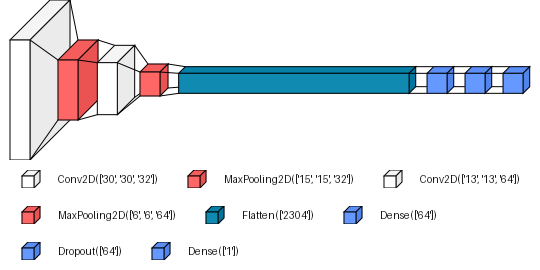
\includegraphics[width=0.9\textwidth]{cnn_architecture.png}
  \caption{Schematic of the proposed CNN architecture.}
  \label{fig:architecture}
\end{figure}

\begin{figure}[p]
  \centering
  \includegraphics[width=0.9\textwidth]{learning_curves.png}
  \caption{Training and validation accuracy / loss curves.}
  \label{fig:learning}
\end{figure}

\end{document}